\documentclass[letterpaper,11pt]{article}
\oddsidemargin -1.0cm \textwidth 17.5cm

\usepackage[utf8]{inputenc}
\usepackage[activeacute,spanish, es-lcroman]{babel}
\decimalpoint
\usepackage{amsfonts,setspace}
\usepackage{amsmath}
\usepackage{amssymb, amsmath, amsthm}
\usepackage{comment}
\usepackage{float}
\usepackage{amssymb}
\usepackage{dsfont}
\usepackage{anysize}
\usepackage{multicol}
\usepackage{enumerate}
\usepackage{graphicx}
\usepackage[left=1.5cm,top=2cm,right=1.5cm, bottom=1.7cm]{geometry}
\setlength\headheight{1.5em} 
\usepackage{fancyhdr}
\usepackage{multicol}
\usepackage{hyperref}
\usepackage{wrapfig}
\usepackage{subcaption}
\usepackage{siunitx}
\usepackage{cancel}
\usepackage{mdwlist}
\usepackage{svg}
\usepackage{tcolorbox}
\usepackage{soul}
\pagestyle{fancy}
\fancyhf{}
\renewcommand{\labelenumi}{\normalsize\bfseries P\arabic{enumi}.}
\renewcommand{\labelenumii}{\normalsize\bfseries (\alph{enumii})}
\renewcommand{\labelenumiii}{\normalsize\bfseries \roman{enumiii})}


\begin{document}

\fancyhead[L]{\itshape{Facultad de Ciencias F\'isicas y Matem\'aticas}}
\fancyhead[R]{\itshape{Universidad de Chile}}

\begin{minipage}{11.5cm}
    \begin{flushleft}
        \hspace*{-0.6cm}\textbf{FI1000-1 Introducción a la Física Clásica}\\
        \hspace*{-0.6cm}\textbf{Profesora:} Jocelyn Dunstan\\
        \hspace*{-0.6cm}\textbf{Auxiliar:} Alejandro Silva\\
        \hspace*{-0.6cm}\textbf{Ayudantes:} Macarena Muñoz \& Catalina Vargas\\
    \end{flushleft}
\end{minipage}

\begin{picture}(2,3)
    \svgpath{../}  % descomentar si se agrega a carpeta "auxiliares"/"ejercicios"
    \put(366, 10){\includesvg[scale=0.31]{img/dfi.svg}}
\end{picture}

\begin{center}
	\LARGE\textbf{Auxiliar \#12}\\
	\Large{Estática del sólido \st{b}rígido}
\end{center}

\vspace{-1cm}
\begin{enumerate}\setlength{\itemsep}{0.4cm}

\rfoot[]{pág. \thepage}

\item[]

\item

Una barra de masa $M$ y largo $L$, que puede pivotear libremente en torno a $O$, se mantiene en equilibrio con una masa $m$ y una cuerda, tal como se muestre en la figura. Encuentre el ángulo $\alpha$ para el caso en que $m/M=0.5$

\begin{figure}[H]
    \centering
    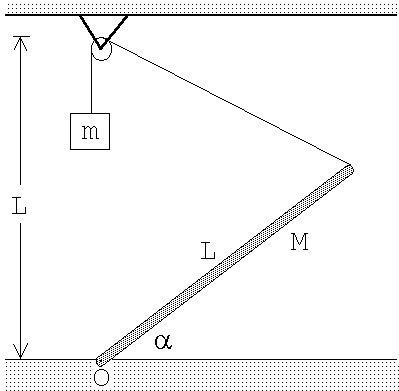
\includegraphics[width=0.25\linewidth]{2021-2/img/aux12/aux12-barra-polea.png}
\end{figure}

\item Una tortuga de masa $m$ camina con velocidad constante $v_0$ sobre una barra de largo $L$ y masa $M$. La barra cuelga de sus extremos por cuerdas verticales sin masa. En $t=0$ la tortuga está en el extremo izquierdo de la barra.
    \begin{enumerate}
        \item Determine las tensiones de las cuerdas en función del tiempo
        
        \item Suponga que la cuerda de la izquierda es de acero, pero la de la derecha es un hilo común. Por eso, la cuerda de la derecha tiene una tensión de corte de $T_{max}$, ¿cuál es la distancia máxima que puede recorrer la tortuga sin que se caiga?
    \end{enumerate}
    
\begin{figure}[H]
    \centering
    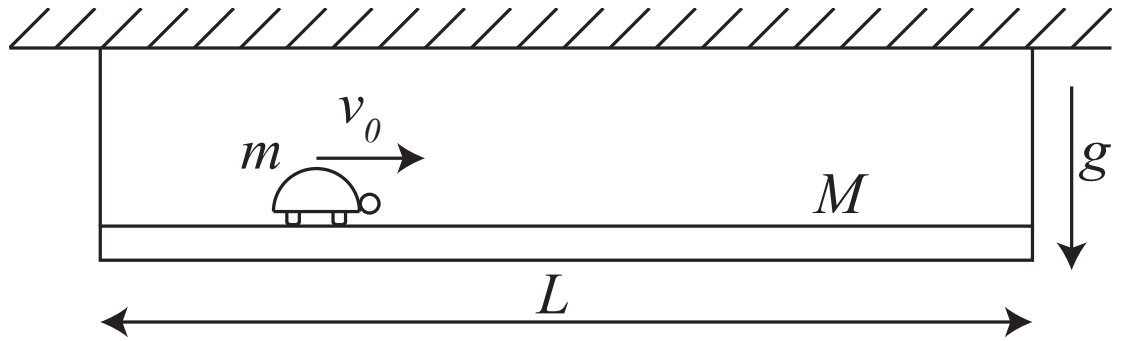
\includegraphics[width=0.45\linewidth]{2021-2/img/aux12/aux12-tortuga.PNG}
\end{figure}

\item 
\begin{multicols}{2}
    Una barra de masa $M$ y largo $L$, con densidad de masa uniforme, se apoya sobre un círculo de radio $R$. Entre la barra y el círculo no hay roce, mientras que entre la barra y el suelo hay roce. Si la barra forma un ángulo $\alpha$ con el suelo, calcule el rango de valores del coeficiente de roce estático $\mu_e$ que permiten que la barra esté en equilibrio estático
    \columnbreak
    \begin{figure}[H]
        \centering
        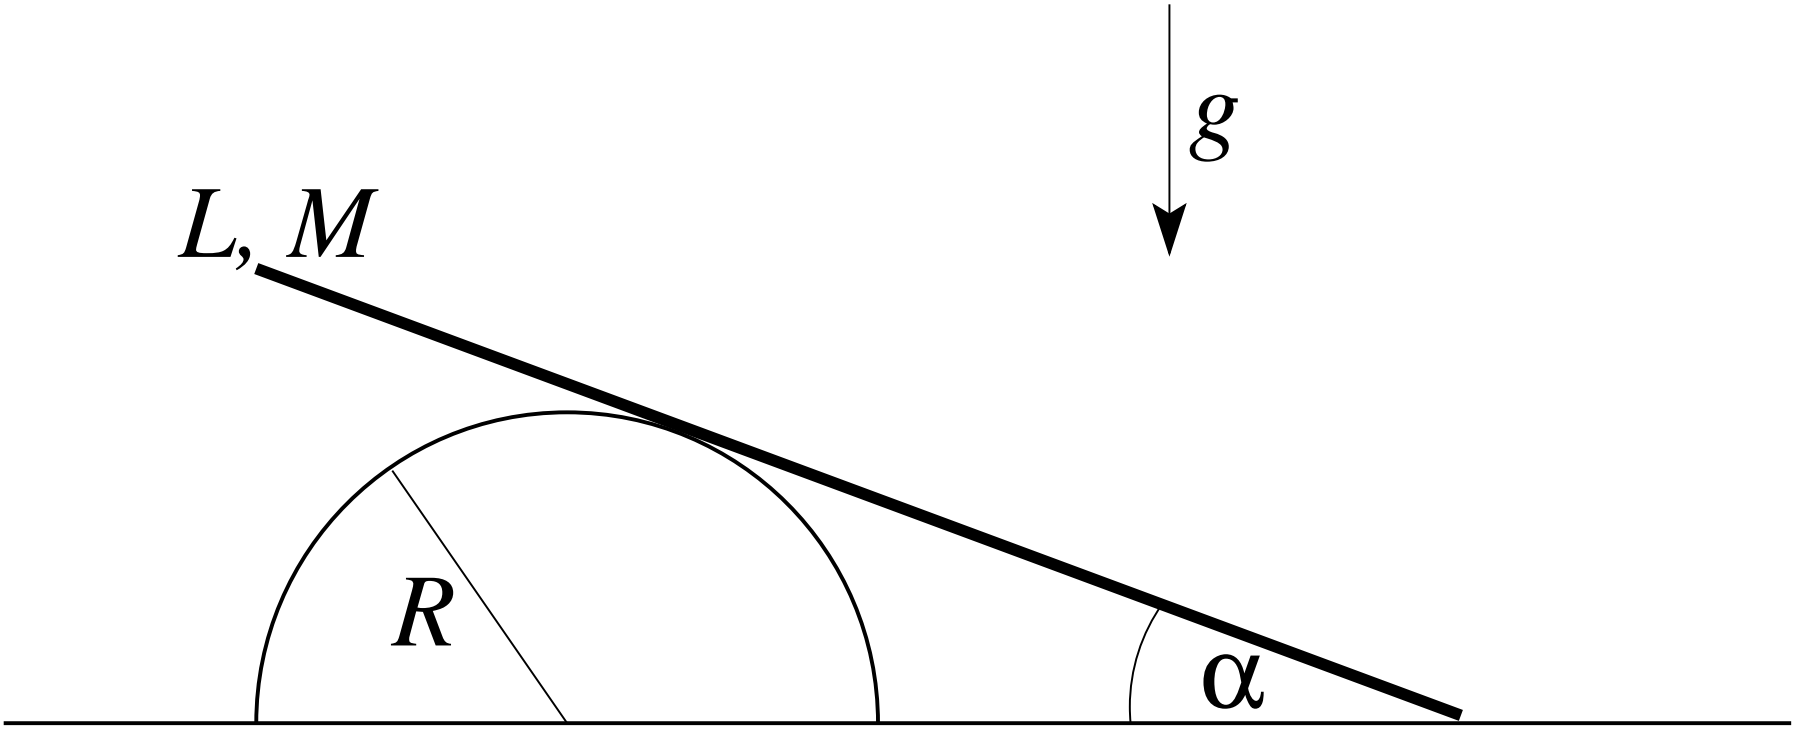
\includegraphics[height=6.5\baselineskip]{2021-2/img/aux12/aux12-circ.PNG}
    \end{figure}
\end{multicols}

% Para imágenes vectoriales -> el texto tiene que estar en LaTeX
% \begin{figure}[htbp]
%   \centering
%   \svgpath{../Imagenes/ejercicios}  -> .. irse pa'trás 
%   \includesvg{ej5.svg}
% \end{figure}

\end{enumerate}
\end{document}